\chapter{Analytic model of nondegenerate internal squeezing} %Research chapter: ...
\label{chp:nIS_analytics}

% results: interpret deep and far, and be very critical of assessing your approach
% present analysis of model and decisions/approximations made
% think about the story!
% systematic and diligent
% wring all of the information out of the results/figures, find the importance and the physics

% separate this into multiple .tex files once structure finalised

%%%%%%%%%%%%%%%%%%%%%%%%%%%%%%%%%%%%%%%%%%
% chapter introduction

\jam{(Fix up mentions of nondegenerate internal squeezing in background chapters, either explain it earlier or do not confuse the reader)}

% combine the all-optical approach of dIS with the mode structure of sWLC
In this chapter, I present my analytic, Hamiltonian model of nondegenerate internal squeezing and the immediate results from it. Nondegenerate internal squeezing is the same configuration as degenerate internal squeezing except that the squeezer is operated nondegenerately, but it is better thought of as an all-optical alternative to stable optomechanical filtering. Firstly, I will review the limited literature available about nondegenerate internal squeezing, and conclude that the system with optical loss has never been fully characterised. Secondly, I will present my model and derive the sensitivity of the configuration. Thirdly, I will partially verify the model by demonstrating that it obeys the expected low and high loss limits. Fourthly, I will show that the system is stable by examining the zeros of the transfer functions' denominator. And finally, motivated by the sensitivity analysis, I will derive the threshold of the lossy configuration using an observation that unites the different squeezing configurations in this thesis. 
% from the view of quantum optics, gravitational waves in the next chapter
This chapter is written from the perspective of understanding nondegenerate internal squeezing for general quantum metrology. In the following chapters, I will return to the problem of kilohertz gravitational-wave detection and whether nondegenerate internal squeezing can feasibly improve sensitivity. 


\section{Literature review}
% a gap in the literature, should be much shorter than the review in Section~\ref{sec:literature_review} -- maybe combine it with that one?
% cannot cite personal communication?
% claim: the modelling of this configuration has never been done as thoroughly as my work, explain why (recency of interest)

\jam{(How to be thorough with this section?)}

The available literature about nondegenerate internal squeezing is limited. Although nondegenerate OPOs have long been studied for tests of the EPR-paradox~\cite{Reid1989,Schori2001} and other applications~\cite{,,}, placing a nondegenerate squeezer in a coupled cavity system \jam{has only been studied in ... (I am not aware of any other mentions than Li 2020, need to read up and ask the supervisors.)}. 
The two configurations in the previous chapter which motivate nondegenerate internal squeezing have only recently \jam{(quantify this?)} been studied, see Section~\ref{sec:literature_review}, and a study of nondegenerate internal squeezing seems inevitable to follow from combining those configurations. \jam{(Is there direct mention of nIS in the dIS literature?)}
The only direct mention of nondegenerate internal squeezing \jam{(that I could find, check this!)} in the literature is the brief suggestion in Ref.~\cite{Li2020} that it is equivalent to stable optomechanical filtering in the lossless case. In that paper, and subsequent work by the same authors~\cite{Li2021}, only mechanical loss is included in the model since it is the dominant source of loss. By the modal equivalence, I predict that optical loss in the idler mode should be the dominant source of loss for nondegenerate internal squeezing, but this is not guaranteed because the behaviour of mechanical and optical loss is different~\cite{} \jam{(is it? but same Langevin terms?)}. I identify this as a gap in the literature, no work has fully characterised the behaviour of the three mode system in the presence of optical loss in every mode, which matters because the distribution of loss in applications might be far from uniform, e.g.\ how the detection loss is predicted to be higher than any of the intra-cavity losses for future gravitational-wave detectors~\cite{}. By a full characterisation, I mean that not only is the quantum noise and signal response of the lossy system not available, but aspects important to understanding the system, such as its limits and the squeezing threshold, are not known. I will address this gap \jam{(be more precise?)}.


\section{Analytic model}

\jam{(Compare to appendices and see if all information is present, then delete appendices (version control will save you))}

\begin{figure}
	\centering
	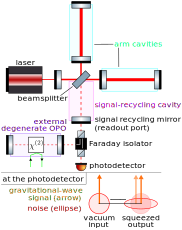
\includegraphics[width=\textwidth]{nIS_config.pdf}
	% squeezing ellipse and signal arrow plot
	\caption{\jam{(Purpose: explain configuration)} \jam{(Draft figure. Needs idler mode and mode labels, integrate figures on right into configuration.)} Nondegenerate internal squeezing configuration with all modes labelled. Explaining the system's response using the signal arrow and noise ellipse representation from Fig.~\ref{fig:extSqz_config}.}
	\label{fig:nIS_config}
\end{figure}

Nondegenerate internal squeezing consists of a nondegenerate squeezer placed inside the signal-recycling cavity of an interferometer, as shown in Fig.~\ref{fig:nIS_config} \jam{(have said this a few times already)}. In the single-mode approximation, I consider the signal and idler modes resonant in the signal-recycling cavity, where the signal mode of the squeezer is at the carrier frequency $\omega_0$ and is resonant in the arms, while the idler mode at $\omega_0+\Delta$ is assumed not resonant in the arms. 
I model this configuration using the Hamiltonian method demonstrated several times in this thesis, where this model combines the nondegenerate OPO model in Section~\ref{sec:nOPO} and the degenerate internal squeezing model in Section~\ref{sec:dIS_model}. There are no steps that have not already appeared in this thesis. This model is also based on and verified against Ref.~\cite{Li2020} in the lossless case. 
% \jam{(Probably need to talk about my methodology more -- state that this derivation presented is the last of a long line of increasing complexity (more losses, radiation pressure, pump phase, etc.) and that I have verified at each stage that the model recovers the previous model. This allowed me to also consider the impact of each subsequent addition in isolation. Moreover, I should re-emphasise that it reduces to the lossless case in Li and follows the same path as the verified models of dIS and the OPOs. The point is that this derivation is not controversial.)}
My methodology when constructing this model was to progressively add each complication to the lossless model in Ref.~\cite{Li2020}, such as optical loss in each mode, radiation pressure, and pump phase. At each stage, I verified that the model recovered the previous stage in the appropriate limits. This allowed me to study the effect of each complication one at a time, however, re-deriving the sensitivity each time was inefficient. I understand the sensitivity by looking at the signal and noise responses separately, and show all three whenever possible. \jam{(need to be more critical of the approach?)} I present the complete model here for brevity.

Let the modes be labelled as shown in Fig.~\ref{fig:nIS_config}, i.e.\ as in Section~\ref{sec:dIS_model} but with the addition of $\hat c$ for the idler mode as in Section~\ref{sec:nOPO}. The Hamiltonian of this system is $\hat H = \hat H_0 + \hat H_I + \hat H_\gamma + \hat H_\text{GW}$ where~\cite{} \jam{(fill in Langevin Hamiltonian)}
\begin{align}
\hat H_0 &= \hbar \omega_0 \hat a^\dag \hat a + \hbar \omega_0 \hat b^\dag \hat b+ \hbar (\omega_0+\Delta) \hat c^\dag \hat c + \hbar (2\omega_0+\Delta) \hat u^\dag \hat u\\
\hat H_I &= i\hbar\omega_s(\hat a\hat b^\dag-\hat a^\dag\hat b) + \hbar \frac{x}{2} (e^{i\phi} \hat u \hat b^\dag \hat c^\dag+e^{-i\phi} \hat u^\dag \hat b \hat c) \\
\hat H_\gamma &= \int \ldots \\
\hat H_\text{GW} &= -\alpha (\hat{x}-L_\mathrm{arm}h(t))\left(\frac{\hat{a}+\hat{a}^\dag}{\sqrt{2}}\right)+\frac{1}{2\mu}\hat{p}^2.
\end{align}
As before, $\hat H_0$ describes the decoupled optical system, $\hat H_I$ describes the interaction between the three intra-cavity modes, $\hat H_\gamma$ describes the input/output coupling through the readout and loss ports listed below, and $\hat H_\text{GW}$ describes the coupling to the gravitational-wave signal and the evolution of the test mass mechanical mode.
There is vacuum entering the system intra-cavity to all three modes $\hat n^L_a, \hat n^L_b, \hat n^L_c$, at the readout port $\hat B_\text{in}, \hat C_\text{in}$, and in the detection chain $\hat n^L_\text{PD}$ which will be included later. Only the vacuum entering the readout port is present in the lossless model.
The Heisenberg-Langevin equations-of-motion for these operators can be found as before, using the bosonic and canonical commutation relations with all other commutators zero. I again (1) make the semi-classical and no-pump-depletion approximations to simplify the pump mode $\hat u\mapsto u=2\chi/x$, these approximations are valid below threshold, (2) enter the Interaction Picture to ignore $\hat H_0$, and (3) take fluctuating components of each operator but keep it implicit in the notation because it does not change the equations-of-motion \jam{(prove this?)}. I find the equations-of-motion to be
\begin{equation}\label{eq:nIS_EoM}
\begin{cases}
\dot{\hat{a}}=-\omega_s\hat{b} - \gamma_a \hat{a} + \sqrt{2\gamma_a}\hat{n}^L_a+\frac{i}{\hbar}\alpha(\hat{x}-L_\mathrm{arm}h)\frac{1}{\sqrt{2}}\\
\dot{\hat{b}}=\omega_s\hat{a} - i\chi e^{i\phi}\hat{c}^\dagger - \gamma^b_\mathrm{tot} \hat{b} + \sqrt{2\gamma^b_R}\hat{B}_\mathrm{in} + \sqrt{2\gamma_b}\hat{n}^L_b\\
\dot{\hat{c}}=-i\chi e^{i\phi}\hat{b}^\dagger - \gamma^c_\mathrm{tot} \hat{c} + \sqrt{2\gamma^c_R}\hat{C}_\mathrm{in} + \sqrt{2\gamma_c}\hat{n}^L_c\\
\dot{\hat{x}}=\frac{1}{\mu}\hat{p}\\
\dot{\hat{p}}=\alpha\left(\frac{\hat{a}+\hat{a}^\dag}{\sqrt{2}}\right).
\end{cases}
\end{equation}
I solve these equations in the Fourier domain with simplified notation $\tilde{\delta\hat{Q}}(\Omega)\mapsto\hat{Q}(\Omega)$. Let $\vec{\hat b}(\Omega)=[\hat b(\Omega), \hat b^\dag(-\Omega), \hat c(\Omega), \hat c^\dag(-\Omega)]^\text{T}$ with similar signal-idler vectorisation for each other mode as in Section~\ref{sec:nOPO} and $\vec{\hat a}(\Omega)=[\hat a(\Omega), \hat a^\dag(-\Omega),0,0]^\text{T},\quad \vec h(\Omega)=\tilde h(\Omega) [1,1,0,0]^\text{T}$ and similarly for $\vec{\hat n}^L_a(\Omega)$. Solving the resulting algebraic equations, I find that
\begin{align}
\mathrm{M}_b\vec{\hat{b}}(\Omega)&= \omega_s\begin{bsmallmatrix}
1 &  &  &  \\
 & 1 &  &  \\
 &  & 0 &  \\
 &  &  & 0
\end{bsmallmatrix}\mathrm{M}_a^{-1}\left(\sqrt{2\gamma_a}\begin{bsmallmatrix}
1 &  &  &  \\
 & 1 &  &  \\
 &  & 0 &  \\
 &  &  & 0
\end{bsmallmatrix}\vec{\hat{n}}^L_a(\Omega)-i\beta\begin{bsmallmatrix}
1 &  &  &  \\
 & -1 &  &  \\
 &  & 0 &  \\
 &  &  & 0
\end{bsmallmatrix}\vec{h}(\Omega)\right)\\&+ \sqrt{2}\begin{bsmallmatrix}
\sqrt{\gamma^b_R} &  &  &  \\
 & \sqrt{\gamma^b_R} &  &  \\
 &  & \sqrt{\gamma^c_R} &  \\
 &  &  & \sqrt{\gamma^c_R}
\end{bsmallmatrix}\vec{\hat B}_\mathrm{in}(\Omega) + \sqrt{2}\begin{bsmallmatrix}
\sqrt{\gamma_b} &  &  &  \\
 & \sqrt{\gamma_b} &  &  \\
 &  & \sqrt{\gamma_c} &  \\
 &  &  & \sqrt{\gamma_c}
\end{bsmallmatrix}\vec{\hat n}^L_b(\Omega)\\
\mathrm{M}_a &= (\gamma_a-i\Omega)\mathrm{I}+\frac{i\rho}{\Omega^2 \sqrt{2}}\begin{bsmallmatrix}
1 & 1 &  &  \\
-1 & -1 &  &  \\
 &  & 0 &  \\
 &  &  & 0
\end{bsmallmatrix}\\
\text{M}_b&=\begin{bsmallmatrix}
\gamma^b_\mathrm{tot} &  &  &  \\
 & \gamma^b_\mathrm{tot} &  &  \\
 &  & \gamma^c_\mathrm{tot} &  \\
 &  &  & \gamma^c_\mathrm{tot} 
\end{bsmallmatrix}-i\Omega \text{I}+\chi \begin{bsmallmatrix}
0 &  &  & i e^{i\phi} \\
 & 0 & -i e^{-i\phi} &  \\
 & i e^{i\phi} & 0 &  \\
-i e^{-i\phi} &  &  & 0
\end{bsmallmatrix}+\omega_s^2\begin{bsmallmatrix}
1 &  &  &  \\
 & 1 &  &  \\
 &  & 0 &  \\
 &  &  & 0
\end{bsmallmatrix}\text{M}_a^{-1}\begin{bsmallmatrix}
1 &  &  &  \\
 & 1 &  &  \\
 &  & 0 &  \\
 &  &  & 0
\end{bsmallmatrix}.
\end{align}
Where $\beta, \rho$ are given by Eq.~\ref{eq:beta_and_rho}, $\text{I}$ is the 4 by 4 identity matrix, and all off-diagonal terms in each matrix are zero unless otherwise shown \jam{(is this clear or would it be better to include them explicitly?)}. Using $\Gamma= \frac{1}{\sqrt2}\begin{bsmallmatrix}
1 & 1 &  &  \\
-i & i &  &  \\
 &  & 1 & 1 \\
 &  & -i & i
\end{bsmallmatrix}$ and the input/output relations at the readout port and the detection loss port given by Eq.~\ref{eq:nOPO_IO_relations}, I find the signal and idler quadratures~\footnote{Where $\vec{\hat X}(\Omega)=[\hat X_{b,1}(\Omega),\hat X_{b,2}(\Omega),\hat X_{c,1}(\Omega),\hat X_{c,2}(\Omega)]^\text{T}$, as in Section~\ref{sec:nOPO}.} at the photodetector to be
\begingroup
\allowdisplaybreaks
\begin{align}
\vec{\hat X}_\mathrm{PD}(\Omega)&=\text{T}\vec h(\Omega)+\text{R}_\text{in}\vec{\hat X}_\mathrm{in}(\Omega)+\text{R}^L_a\vec{\hat X}^L_a(\Omega)+\text{R}^L_b\vec{\hat X}^L_b(\Omega)+\text{R}^L_\text{PD}\vec{\hat X}^L_\text{PD}(\Omega)\\
\text{T}&=-\sqrt{1-R_\text{PD}}\omega_s(-i\beta)\Gamma \sqrt{2}\begin{bsmallmatrix}
\sqrt{\gamma^b_R} &  &  &  \\
 & \sqrt{\gamma^b_R} &  &  \\
 &  & \sqrt{\gamma^c_R} &  \\
 &  &  & \sqrt{\gamma^c_R}
\end{bsmallmatrix}\text{M}_b^{-1}\begin{bsmallmatrix}
1 &  &  &  \\
 & 1 &  &  \\
 &  & 0 &  \\
 &  &  & 0
\end{bsmallmatrix}\text{M}_a^{-1}\begin{bsmallmatrix}
1 &  &  &  \\
 & -1 &  &  \\
 &  & 0 &  \\
 &  &  & 0
\end{bsmallmatrix}\\
\text{R}_\text{in}&=\sqrt{1-R_\text{PD}}\Gamma\left(\text{I}-2\begin{bsmallmatrix}
\sqrt{\gamma^b_R} &  &  &  \\
 & \sqrt{\gamma^b_R} &  &  \\
 &  & \sqrt{\gamma^c_R} &  \\
 &  &  & \sqrt{\gamma^c_R}
\end{bsmallmatrix}\text{M}_b^{-1}\begin{bsmallmatrix}
\sqrt{\gamma^b_R} &  &  &  \\
 & \sqrt{\gamma^b_R} &  &  \\
 &  & \sqrt{\gamma^c_R} &  \\
 &  &  & \sqrt{\gamma^c_R}
\end{bsmallmatrix}\right)\Gamma^{-1}\\
\text{R}^L_a&=-\sqrt{1-R_\text{PD}}\omega_s\Gamma 2\sqrt{\gamma_a}\begin{bsmallmatrix}
\sqrt{\gamma^b_R} &  &  &  \\
 & \sqrt{\gamma^b_R} &  &  \\
 &  & \sqrt{\gamma^c_R} &  \\
 &  &  & \sqrt{\gamma^c_R}
\end{bsmallmatrix}\text{M}_b^{-1}\begin{bsmallmatrix}
1 &  &  &  \\
 & 1 &  &  \\
 &  & 0 &  \\
 &  &  & 0
\end{bsmallmatrix}\text{M}_a^{-1}\begin{bsmallmatrix}
1 &  &  &  \\
 & 1 &  &  \\
 &  & 0 &  \\
 &  &  & 0
\end{bsmallmatrix}\Gamma^{-1}\\
\text{R}^L_b&=-\sqrt{1-R_\text{PD}}\Gamma 2\begin{bsmallmatrix}
\sqrt{\gamma^b_R} &  &  &  \\
 & \sqrt{\gamma^b_R} &  &  \\
 &  & \sqrt{\gamma^c_R} &  \\
 &  &  & \sqrt{\gamma^c_R}
\end{bsmallmatrix}\text{M}_b^{-1}\begin{bsmallmatrix}
\sqrt{\gamma^b_R} &  &  &  \\
 & \sqrt{\gamma^b_R} &  &  \\
 &  & \sqrt{\gamma^c_R} &  \\
 &  &  & \sqrt{\gamma^c_R}
\end{bsmallmatrix}\Gamma^{-1}\\
\text{R}^L_\text{PD}&=\sqrt{R_\text{PD}} \text{I}.
\end{align}
\endgroup
The total quantum noise is given by the spectral density matrix Eq.~\ref{eq:total_noise_matrix}, which simplifies, assuming uncorrelated vacuum at each loss port, to
\begin{equation}
\text{S}_X=\text{R}_\text{in}\text{R}_\text{in}^\dag+\text{R}^L_a{\text{R}^L_a}^\dag+\text{R}^L_b{\text{R}^L_b}^\dag+\text{R}^L_\text{PD}{\text{R}^L_\text{PD}}^\dag.
\end{equation} % same expression as dIS
Which is divided into 2 by 2 blocks of signal-signal, signal-idler, and idler-idler (co)variances as in Section~\ref{sec:nOPO} \jam{(are the s-s and i-i covariances all zero, how many freedoms remaining in the s-i covariances?)}. The pump phase only appears in the off-diagonal, signal-idler blocks.
The vector of signal transfer functions, with respect to $\tilde h(\Omega)$, to each signal and idler quadrature at the photodetector is
\begin{equation}\label{eq:nIS_sigRO_signal_response}
\text{T}\begin{bsmallmatrix}1 \\1\\0\\0\end{bsmallmatrix} = \frac{2 \beta \sqrt{1-R_\text{PD}} \omega_s}{(\gamma_a-i \Omega ) \left(\chi ^2-(\gamma^b_\text{tot}-i\Omega) (\gamma^c_\text{tot}-i\Omega)\right)-\omega_s^2 (\gamma^c_\text{tot}-i \Omega )} \begin{bsmallmatrix}0 \\-\sqrt{\gamma^b_R}(\gamma^c_\text{tot}-i\Omega)\\\sqrt{\gamma^c_R}\chi\cos(\phi)\\\sqrt{\gamma^c_R}\chi\sin(\phi)\end{bsmallmatrix}.
\end{equation}
Therefore, there is gravitational-wave signal in the second signal quadrature and each idler quadrature. For simplicity and to compare to Ref.~\cite{Li2020}, here I will consider measuring the second signal quadrature which I will refer to as signal readout, henceforth. However, this is not necessarily the optimum readout of the signal quadratures since the noise might be sufficiently lower in the first quadrature to preference a combined measurement. I will consider this and other readout schemes, such as measurements of the idler quadratures and combinations of the signal and idler quadratures, like in Section~\ref{sec:nOPO_combined_readout}, in Chapter~\ref{chp:idler_readout}.
Therefore, the sensitivity of the signal readout scheme, where $\sqrt{S_h}$ is the noise-to-signal ratio, is
\begin{equation}\label{eq:nIS_sigRO_sens}
S_h = \frac{(\text{S}_X)_{2,2}}{\abs{\left(\text{T}\begin{bsmallmatrix}1 \\1\\0\\0\end{bsmallmatrix}\right)_2}^2}.
\end{equation}
% verified these results by repeating the model with 2x2 matrices and 4x4 matrices, important to mention this because it is part of the methodology
\jam{(Include full expression in an appendix?)} I have partially verified this result by repeating the derivation using 2 by 2 matrices~\footnote{This is not a physically meaningful difference, but it separates the signal and idler such that the derivations are not identical.}, and will also compare it to known limits below. %in Section~\ref{sec:nOPO_reduction}.


\section{Results}

I will now examine some of the immediate results of the model: (1) the general features of the signal and noise responses and sensitivity, (2) the reduction to known models in certain loss limits, and (3) the stability of the system.

\subsection{General behaviour}
% should this be down in results section? --> this is a results chapter, maybe include a short section discussing the general performance (separate from the science case analysis in chapter 5?)

% plot: classic N, S, NSR; also noise budget plot
% need to show some example plots here to set up those in the next section?
\begin{figure}
	\centering
	\includegraphics[width=\textwidth]{nIS_N_S_NSR.pdf}
	\caption{\jam{(Purpose: Plain plot to discuss the general features of nIS)} \jam{(The legends of these noise-signal-NSR plots need to be fixed so that the plot and text can be larger, perhaps place the legend under the plot.)} Nondegenerate internal squeezing signal readout with losses, showing quantum noise response (top panel), signal response (middle panel), and sensitivity (bottom panel). The effect of the squeezer and radiation pressure are shown. The slope of the radiation pressure noise with the squeezer on appears to change around 10~Hz which is an effect of losses, the same effect causes the signal to not be amplified down to DC. \jam{(explain that threshold is explained later)}}
	\label{fig:nIS_general_sens}
\end{figure}

\jam{(should I instead show the lossless limit first?)}

% analyse typical nIS plot features before getting into different tests
The performance of nondegenerate internal squeezing is shown in Fig.~\ref{fig:nIS_general_sens} \jam{(for what parameters?)}. 
With the squeezer off, the sensitivity curve is shaped by the radiation-pressure noise below 10~Hz and the signal response resonance at the sloshing frequency 5~kHz with bandwidth 500~Hz determined by the signal readout rate $\gamma^b_R$, as discussed in Section~\ref{sec:dIS_results}. With the squeezer turned on, (1) the shot noise is anti-squeezed around a frequency determined by the squeezer parameter, sloshing frequency, and loss rates; (2) the radiation-pressure noise worsens to now dominate below 100~Hz; and (3) the signal is amplified around the same frequency as the shot noise and at frequencies down to 10~Hz, below which it converges to the squeezer-off value due to losses. These changes mean that the squeezer improves the sensitivity from 40--4000~Hz and worsens it outside that band except above 10~kHz where the sensitivity is the same \jam{(quantify sameness?)}.
These quoted frequencies are specific to this parameter set but the general performance is the same: nondegenerate internal squeezing leads to improved sensitivity at some broad range of ``middle'' frequencies at the cost of ``low'' frequency sensitivity. 
Some of these effects will be explained later: the frequency around which the shot noise and the signal peak are amplified will be determined by the threshold of the system and the effect of losses will be left until I consider gravitational-wave detection feasibility. But, some of these results can be understood immediately.
% changing the signal response via the white-light cavity effect?
% why aren't the changes local to the sloshing frequency, like dIS?
The signal response is amplified by analogy to the filter (white-light) cavity effect of the optomechanical analogue, the resonance of the coupled cavity system is changed by introducing the idler mode \jam{(is this true? I am not sure. the signal response still falls off at the same rate so bandwidth doesn't seem to improve except by the LF amplification?)}. The change in the resonance behaviour from a two-mode to a three-mode coupled system means that the changes are not localised to the sloshing frequency, unlike degenerate internal squeezing in Section~\ref{sec:dIS_results} \jam{(but shouldn't this mean that they are still expected around the coupling frequencies?)}. 
%In the simple explanation of the signal-recycling cavity reflecting the light back into the arms to experience the gravitational wave more, the addition of the idler mode, which is not directly coupled to the arms or measured, somehow \jam{(how/why? this is wishy-washy)}.
% why does radiation pressure noise worsen?
Therefore, the radiation pressure noise can also be affected~\footnote{I only talk about the radiation pressure noise where it is dominant, i.e.\ at ``low'' frequencies below the Standard Quantum Limit \jam{(is this necessary to say?)}.}, it is anti-squeezed \jam{(why does the other quadrature appear now? is it worsened proportionally to the pump power?)}.

\begin{figure}
	\centering
	\includegraphics[width=\textwidth]{nIS_sigRO_noise_budget.pdf}
	\caption{\jam{(Purpose: Want to show how the different noises look.)} \jam{(Should make plot below threshold, fix the idler loss, show lower frequencies.)} Nondegenerate internal squeezing breakdown of quantum noise response to different sources, plotting separate noise transfer functions for each loss port (this is akin to a typical ``noise budget''~\cite{} \jam{(what's the difference?)}). The detection loss affects the shot noise after the interferometer, and therefore is flat. The other losses are all squeezed and affected by the radiation-pressure noise \jam{(show lower frequencies to show readout loss RPN)}. The readout port dominates the other losses, followed by the idler intra-cavity loss.}
	\label{fig:nIS_sigRO_noise_budget}
\end{figure}

\jam{(I do not understand why the radiation pressure is anti-squeezed where it was not affected in dIS, see possible explanation above. Also, why is RPN anti-squeezed in the lossless case?)}

To better understand the radiation pressure noise, I consider how it appears in each of the contributions to the total quantum noise, shown in Fig.~\ref{fig:nIS_sigRO_noise_budget}. The effect of each loss will be examined in detail in the next chapter. The radiation pressure noise appears in the contribution from the readout port and each intra-cavity loss port. This is because the radiation pressure noise, with the gravitational-wave signal, enters the measured, second signal quadrature after the input test mass. Having already seen the arm cavity loss, it gets added here to each of the noises that travel through the signal mode \jam{(what am I trying to say?)}. It is then anti-squeezed \jam{(check this)} and read out. \jam{(why is the shot noise not amplified at LF, I need to resolve this.)}

% explain the effect of each parameter? (except leave tolerance to losses to science case chapter)
\jam{(is this necessary? true? complete?)}
The effect of each interferometer parameter is similar to the no-squeezing case of the two-cavity system, which is contained in Sections~\ref{sec:intro_IFO}~\ref{sec:dIS_results}. To summarise, in terms of the configuration parameters rather than derived parameters such as the sloshing frequency and readout rates, increasing the circulating power in the arms increases the sensitivity at all frequencies. Increasing the arm length increases the same scalar factor as the power, reduces the free-spectral range of the signal response (i.e.\ the signal response falls off at a lower frequency), and decreases the sloshing frequency (and therefore the peak of the squeezed system). The sloshing frequency also decreases with decreased input test mass transmission and a longer signal-recycling cavity. Increasing the signal-recycling length decreases the bandwidth of the signal peak \jam{(Are there two bandwidths? The FSR of the arms sets where the signal falls off and the readout rate sets the smaller bandwidth around the sloshing frequency peak?)}, which is also decreased by decreased signal-recycling mirror transmission. The radiation-pressure noise increases with heavier test masses and increased pump power (squeezer parameter). Finally, increased pump power also increases the peak shot noise and signal amplification, and the pump phase does not affect signal readout. \jam{(I am claiming a lot here without figures or citations, what to include?)}


\subsection{Reduction to known systems}

% show that this follows from the EoM but can be verified by looking at the plots
To partially verify the model, I show that it reduces to the expected limits when (1) the losses are removed and (2) the arm loss is taken to infinity. I predict the behaviour by taking the limits of the equations-of-motion in Eq.~\ref{eq:nIS_EoM} and verify it by examining the plots of the noise and signal responses.

\subsubsection{Lossless limit}

\begin{figure}
	\centering
	\includegraphics[width=\textwidth]{nIS_lossless.pdf}
	\caption{\jam{(Purpose: show limit 1/2)} \jam{(Need to add lossless limit to compare to. Use code from Li et al 2020, Fig 5)} Nondegenerate internal squeezing noise, signal, and sensitivity, showing the lossless limit compared to the lossless optomechanical analogue from Fig.~\ref{fig:sWLC_sensitivity} which has no idler readout rate. Compare to the lossy plots in Fig.~\ref{fig:nIS_general_sens}.}
	\label{fig:nIS_lossless}
\end{figure}

In the lossless limit, $\gamma_a=\gamma_b=\gamma_c=R_\text{PD}=0$, with the idler readout rate turned off, $\gamma^c_R=0$, the equations-of-motion of nondegenerate internal squeezing reduce to those of the lossless optomechanical analogue in Ref.~\cite{Li2020}. Comparing the resulting noise, signal, and sensitivity, shown in Fig.~\ref{fig:nIS_lossless}, \jam{the signal transfer function and the radiation-pressure noise do not agree with the predicted limit. The signal transfer function in Eq.~\ref{eq:nIS_sigRO_signal_response} requires a factor $\sqrt2$ and the test mass requires a factor $2$. (why? fix this. on whose side is the error? does my method of signal transfer function agree with Korobko?)} But if these factors are included then the system reduces to the correct limit.
I will compare the lossy all-optical and optomechanical analogues in the next chapter. 
% no losses means no antisqueezing of shot noise but yes RPN, why? threshold=0 problem?
Without losses, the shot noise is not anti-squeezed and the signal amplification persists down to DC. To explain the former, if the idler readout rate is zero and there is no loss, then the threshold is poorly defined since there is no mechanism for light to leave the idler mode, which will be discussed later. However, taking the limit of smaller and smaller losses does show that the shot noise peak decreases for fixed pump power \jam{(why?)}. The DC signal amplification is lost when losses are added because \jam{(... why? should plot lossless and lossy curves together)}.


\subsubsection{High arm loss limit}
\label{sec:nOPO_reduction}

\begin{figure}
	\centering
	\includegraphics[width=\textwidth]{nIS_nOPO_limit.pdf}
	\caption{\jam{(Purpose: show limit 2/2)} \jam{(Show fewer lines, fix title, y-axis label, but legend is good.)} Nondegenerate internal squeezing shot noise response $\sqrt{(\text{S}_X)_{2,2}|_{\rho=0}}$ showing the large arm loss limit compared to the variance from a nondegenerate OPO with the input test mass fully reflective.}
	\label{fig:nIS_signal_nOPO_limit}
\end{figure}

% full 4x4 matrix agrees, not just variance 1,1
% give best explanation of ITM T=0, but can admit that while the maths is clear the physics is not obvious -- potentially requires more thought
In the high arm loss limit, $\gamma_a\rightarrow\infty$, the equations-of-motion of nondegenerate internal squeezing reduce to those of a nondegenerate OPO with the input test mass fully reflective. Comparing the shot noise of both systems, Fig.~\ref{fig:nIS_signal_nOPO_limit} shows that they converge in the limit, which also holds for the full shot noise matrix $\text{S}_X$ by inspection. This is similar to how the shot noise of degenerate internal squeezing converges to that of a degenerate OPO with the input test mass fully reflective, see Fig.~\ref{fig:dIS_limit_dOPO}, where the same explanation as Section~\ref{sec:dIS_optical_loss} holds for why the mirror is fully reflective. 

% therefore mystery of the idler loss carries over: idler loss cannot be zero
Therefore, the behaviour of nondegenerate internal squeezing, for a given set of parameters, is somewhere between that of the lossless optomechanical analogue and a nondegenerate OPO. And so, I expect certain feature to be inherited from these systems, such as how the above problem with threshold when idler loss is zero is inherited from the nondegenerate OPO threshold in Section~\ref{sec:nOPO_results}.


\subsection{Stability}
\label{sec:nIS_stability}

% plot: imaginary part of poles
\begin{figure}
	\centering
	\includegraphics[width=\textwidth]{nIS_stability.pdf}
	\caption{\jam{(Purpose: show stability)} \jam{(Fix x-axis to threshold normalised. Omit showing real part?. Does this stability plot make sense? Supervisors requested Nyquist plots etc.\ at some point, is that still necessary?)} Stability of nondegenerate internal squeezing, for lossless and lossy cases. Showing the imaginary part of the poles of the transfer functions, when the imaginary part becomes positive the system becomes unstable~\cite{}. The lossless system is stable below threshold. \jam{And the lossy system is ... (find this out)}}
	\label{fig:nIS_stability}
\end{figure}

Stability is a feature of nondegenerate internal squeezing that might not be fully inherited from its limiting configurations (lossless optomechanical analogue and nondegenerate OPO). I use the same method to determine stability as in Section~\ref{sec:dIS_results} and shown in Fig.~\ref{fig:dIS_stability}. Like in Section~\ref{sec:dIS_results}, the signal and noise transfer functions are rational functions of $\Omega, \chi$ with denominators~\footnote{I state these for the modulus-squared transfer functions, i.e.\ the numerator and denominator in Eq.~\ref{eq:nIS_sigRO_sens}, but the poles, i.e.\ zeros of $q$, do not change under the square root.} given by $q(\Omega,\chi)$ and $\Omega^4 q(\Omega,\chi) q(\Omega,-\chi)$, respectively, except that here $q$ only depends on $\chi^2$ and so the noise transfer function denominator is $\Omega^4 q(\Omega,\chi)^2$, where $q$ is some polynomial in $\Omega, \chi$, 
\begin{align}
q(\Omega,\chi)&=\left(\gamma_a^2+\Omega ^2\right) \left(\Omega ^2 \left({\gamma^b_\text{tot}}^2+{\gamma^c_\text{tot}}^2+2 \chi ^2\right)+\left({\gamma^b_\text{tot}} {\gamma^c_\text{tot}}-\chi ^2\right)^2+\Omega ^4\right)\\
&-2 \omega_s^2 \left(\gamma_a {\gamma^c_\text{tot}} \chi ^2-\gamma_a {\gamma^b_\text{tot}} \left({\gamma^c_\text{tot}}^2+\Omega ^2\right)+\Omega ^2 \left({\gamma^c_\text{tot}}^2+\chi ^2+\Omega ^2\right)\right)+\omega_s^4 \left({\gamma^c_\text{tot}}^2+\Omega ^2\right).
\end{align}
This means that the zeros of the transfer functions are the shared zeros of $q$, except for the radiation-pressure noise singularity at $\Omega=0$ which I ignore because it comes from the horizontally free-falling mass assumption and is a pole on the real axis. This is expected because the stability of the system should be the same for the signal and noise \jam{should it? citation?}.
Therefore, nondegenerate internal squeezing is unstable if any of the complex $\Omega$ zeros of $q$ have positive imaginary part. As shown in Fig.~\ref{fig:nIS_stability}, the lossless system is stable for all $\chi\leq\omega_s$ and the lossy system is stable for \jam{... (normalise lossy plot)}. I will show shortly that this means that nondegenerate internal squeezing is stable below threshold, like its two limiting configurations. Because the no-pump-depletion assumption breaks above threshold, the behaviour there cannot be inferred from Fig.~\ref{fig:nIS_stability}.
% non-effect of RP, pump phase
Since $q$ only depends on the pump power, readout and loss rates, and sloshing frequency, other factors, such as radiation pressure or pump phase, do not affect the zeros of $q$ or the stability.


\section{Singularity threshold}
\label{sec:singularity_threshold}
% motivate this by the previous section's looking at poles, now looking at real poles that could be encountered, to avoid confusion with the complex poles that are always present I will call these real poles ``singularities''

% \jam{(Emphasise that this is original work and that it is a clever approach.)}
As established in Sections~\ref{sec:dOPO_threshold}~\ref{sec:nOPO_results}~\ref{sec:dIS_results}, the threshold of a squeezing system is the boundary where gains balance losses and near which \jam{(phrasing)} the no-pump-depletion assumption breaks. Knowing threshold is therefore required to understand where this model is valid and experimentally how high the pump power can be raised without beginning lasing. Although threshold is well-understood for the OPOs and lossless degenerate internal squeezing, the threshold of lossy degenerate and nondegenerate internal squeezing is not available in the literature \jam{(check this, how to prove this?)}. In this section, I present my method for determining threshold in all of these models, which uses the no-pump-depletion assumption.
To briefly explain how I devised this method, since lossless degenerate internal squeezing on threshold has a minimum squeezed quadrature of zero, I initially tried to maximise the anti-squeezed quadrature of nondegenerate internal squeezing against $\Omega,\chi$. But performing this numerically encountered division-by-zero errors which prompted me to examine the transfer functions and find the singularities, i.e.\ the real zeros of $q$, analytically. The key insight was then realising that both the OPOs have singularities at $\Omega=0$ in the anti-squeezed quadrature on threshold.

\begin{figure}
    \centering
    \includegraphics[width=\textwidth]{nIS_on_threshold.pdf}
    \caption{\jam{(Purpose: show that singularity threshold actually gives singularities -- is this necessary?)} Nondegenerate internal squeezing noise, signal, and sensitivity when approaching and at threshold. At and above threshold the no-pump-depletion assumption breaks and the transfer functions are singular. The finiteness of the peaks in the noise and signal responses and the appearance of a peak in the sensitivity are due to numerical error and limited sampling \jam{(am I sure about the sensitivity peak?)}. For the on-threshold behaviour of the other configurations in this thesis see Figs.~\ref{fig:dOPO_variances}~\ref{fig:nOPO_variances}~\ref{fig:dIS_sensitivity}~\ref{fig:sWLC_sensitivity}.}
    \label{fig:nIS_on_threshold}
\end{figure}

My method to determine threshold is to define the ``singularity threshold'' as the smallest (real) value of the squeezing parameter such that the anti-squeezed quadrature of the quantum noise has a singularity at some (real) frequency. In particular, I look for points where the anti-squeezed quadrature, i.e.\ any of the diagonal terms of $\text{S}_X$, diverges to infinity in $(\Omega,\chi)\subset\mathbb{R}^2$ space~\footnote{To reduce confusion, I do not call these points poles since, unlike when considering stability, I am restricting $\Omega,\chi$ to be real and therefore the transfer function is not defined on $\mathbb{C}$.}. Since I include the pump phase freedom in my models, $\chi$ is further restricted to be positive.  \jam{(Check this: looking at the imaginary part of the poles for stability and looking for real poles (i.e. poles on the real axis) for threshold are the same solutions, surely?)}
Defining threshold with respect to anti-squeezing is better than squeezing because the singularities of the anti-squeezed quadrature are expected to be robust to losses, unlike the zeros of the squeezed quadrature, as shown in Fig.~\ref{fig:dOPO_variances}. 
I find the (real~\footnote{The reality condition is used to simplify the zeros of $q$, as in the solution for $\chi^2$ there is an imaginary component that, when set to zero, gives the real $\Omega$ solution.}) singularities of the noise transfer function (squared) $S_X$, i.e.\ the zeros of its denominator, for each squeezing configuration in this thesis to be at \jam{(check that $\gamma_c\mapsto\gamma^c_\text{tot}$)}
\begingroup
\allowdisplaybreaks
\begin{align}\label{eq:singularity_threshold}
\text{degenerate OPO}&: \Omega_\text{thr}=0, \chi_\text{thr}=\gamma^b_\mathrm{tot}\\
\text{nondegenerate OPO}&: \Omega_\text{thr}=0, \chi_\text{thr}=\sqrt{\gamma^b_\mathrm{tot}\gamma^c_\text{tot}}\\
\text{degenerate internal squeezing}&:\begin{cases}
\Omega_1=0, \chi_1=\gamma^b_\mathrm{tot}+\frac{\omega_s^2}{\gamma_a};&\gamma_a\neq0\\
\Omega_2=\sqrt{\omega_s^2-\gamma_a^2}, \chi_2=\gamma^b_\mathrm{tot}+\gamma_a;&\omega_s\geq\gamma_a\geq0
\end{cases}\\
\text{nondegenerate internal squeezing}&:\\&\hspace{-5cm}\begin{cases}
\Omega_1=0, \chi_1=\sqrt{\gamma^c_\text{tot}(\gamma^b_\mathrm{tot}+\frac{\omega_s^2}{\gamma_a})};&\gamma^c_\text{tot}\neq0,\gamma_a\neq0\\
\Omega_2=\sqrt{\frac{\gamma^c_\text{tot}\omega_s^2-\gamma_a(\omega_s^2+\gamma_a(\gamma^b_\mathrm{tot}+\gamma^c_\text{tot}))}{\gamma^b_\mathrm{tot}+\gamma^c_\text{tot}}}, \chi_2=\sqrt{(\gamma_a+\gamma^b_\mathrm{tot})(\gamma_a+\gamma^c_\text{tot}+\frac{\omega_s^2}{\gamma^b_\mathrm{tot}+\gamma^c_\text{tot}})};&\gamma^c_\text{tot}\neq0,(*)
\end{cases}\\
(*)&:\gamma^c_\text{tot}\omega_s^2\geq\gamma_a\left(\omega_s^2+\gamma_a(\gamma^b_\mathrm{tot}+\gamma^c_\text{tot})\right)
\end{align}
\endgroup
% frequency around which shot noise and signal are amplified in fig:nIS_general_sens is determined (but not exactly) the threshold frequency
% which pole is chosen tells us the closeness to nOPO or lossless sWLC
Where this result is verified by plotting the results for the given values and observing the singularity, as shown in Fig.~\ref{fig:nIS_on_threshold}. For squeezer parameter just below threshold, e.g.\ $\chi=0.95\chi_\text{thr}$ in Fig.~\ref{fig:nIS_general_sens}, the peak frequency around which the shot noise and signal are amplified is determined by the threshold frequency~\footnote{Consider this peak as a slice with constant $\chi$ of the region around the singularity in (real) $\Omega,\chi$ space.}. If multiple singularities are listed above, the singularity threshold is determined by the smallest $\chi$ value $$\chi_\text{thr}=\min_{i\in\{1,2\}}(\chi_i),\quad\Omega_\text{thr}=\Omega_{\underset{i\in\{1,2\}}{\text{argmin}}(\chi_i)}.$$ Which singularity has the smallest squeezer parameter changes as the losses change, and, by inspection for internal squeezing, where it changes the singularities merge which makes the threshold continuous. This definition is used because it reflects the first singularity hit when the pump power is increased from zero. The merging of the singularities could also be used, informally, as the point where the lossy configuration becomes closer in behaviour to the OPO limit than to the lossless configuration.

\begin{figure}
    \centering
    \includegraphics[width=\textwidth]{dIS_threshold.pdf}
    \caption{\jam{(Purpose: show that concept works for existing system, maybe cut dIS because nIS should be the focus? )} \jam{(Explain the number of extrema)} For degenerate internal squeezing, trajectory of singularities of the anti-squeezed quadrature of noise in $(\Omega, \chi)$ space as losses are changed, as well as trajectory of extrema (assumed as minima) of the squeezed quadrature. Compare to the nondegenerate case in Fig.~\ref{fig:nIS_threshold_traj}. \jam{(explanation moved into text, does it still make sense?)}}
    \label{fig:dIS_threshold_traj}
\end{figure}
\begin{figure}
    \centering
    \includegraphics[width=\textwidth]{nIS_threshold.pdf}
    \caption{\jam{(Purpose: show evolution and limits of threshold)} \jam{(This is confusing, need to annotate the total path discussed in the text, from lossless sWLC to nOPO. Also, change losses to ppm. Fix $\sqrt{\gamma_b\gamma_c}$ label to specify values.)} For nondegenerate internal squeezing, trajectory of singularities of the anti-squeezed quadrature in $(\Omega, \chi)$ space as losses are changed. \jam{(add some explanation back in?)}}
    \label{fig:nIS_threshold_traj}
\end{figure}

Singularity threshold recovers the known threshold values for the OPOs from Sections~\ref{sec:dOPO_threshold}~\ref{sec:nOPO_results} by inspection, degenerate internal squeezing from Section~\ref{sec:dIS_results}, and the optomechanical analogue from Section~\ref{sec:sWLC}. %, but its behaviour with loss is more complex for internal squeezing. 
For degenerate internal squeezing, shown in Fig.~\ref{fig:dIS_threshold_traj}, in the lossless case the singularities $(\Omega,\chi)$ are at $(0,\infty)$ and $(\omega_s,\gamma^b_\text{tot})$ which recovers $(\Omega_\text{thr},\chi_\text{thr})\xrightarrow[\gamma_a\rightarrow0]{}(\omega_s,\gamma^b_\mathrm{tot})$ from Section~\ref{sec:dIS_results}. As the arm loss $\gamma_a$ is increased from zero, the singularities move and merge at the $\Omega=0$ axis when $\gamma_a=\omega_s$, and then the remaining singularity converges to the degenerate OPO threshold $(\Omega_\text{thr},\chi_\text{thr})\xrightarrow[\gamma_a\rightarrow\infty]{}(0,\gamma^b_\mathrm{tot})$ in the high arm loss limit, as expected.
% this resolves the mystery of idler loss --> means that lossless nIS is necessarily above threshold and therefore not allowed in this model except in formal limits, pump depletion would need to be added in to properly compare to sWLC?
For nondegenerate internal squeezing, shown in Fig.~\ref{fig:nIS_threshold_traj} for fixed signal loss $T_{l,b}=0.1$ \jam{(explain)} and no idler readout rate $\gamma^c_R=0$ to compare to the optomechanical analogue, in the lossless limit $\gamma_a=0,\gamma_c\rightarrow0$ the singularities approach $(0,\infty)$ and $(0,\omega_s)$ which recovers the $\chi_\text{thr}=\omega_s$ analogue to the exceptional value $\chi_m=\omega_s$ from Section~\ref{sec:sWLC}. Although this value is not called threshold \jam{(is it not?)} for the optomechanical analogue, the same principle of gains and losses applies to the signal and mechanical idler modes \jam{(justify that these are the same point)}. Moreover, the marginal stability of that system at $\chi_m=\omega_s$ means that a pole in the complex $\Omega$ plane has moved on to the real axis and therefore is a (real) singularity \jam{(clarify that $\chi$ remains real in stability analysis)}. As the idler loss $\gamma_c$ is increased from zero with arm loss $\gamma_a=0$, one singularity remains at $(0,\infty)$ and the other converges to $(\omega_s,\sqrt{\gamma^b_\text{tot}\gamma_c})$ when $\gamma_c\rightarrow\infty$. Fixing the idler loss at $T_{l,c}=0.1$ and now changing the arm loss $\gamma_a$~\footnote{Threshold remains poorly defined when the idler loss is zero \jam{(where is this in the derivation?)} like the nondegenerate OPO in Section~\ref{sec:nOPO_results}. The lossless limit requires $\gamma^c_\text{tot}\rightarrow0$ to be taken formally.}, the singularities merge \jam{(check this)} at the $\Omega=0$ axis when $\gamma^c_\text{tot}\omega_s^2=\gamma_a\omega_s^2+\mathcal{O}(\gamma_a^2)$ which, assuming that $\gamma_a$ is small compared to $\omega_s$~\footnote{Which is reasonable for a gravitational-wave interferometer with $T_{l,a}=100\text{ppm}$ where $\gamma_a/(2\pi)<1$~Hz but $\omega_s/(2\pi)=5$~kHz.}, is approximately when $\gamma_c\approx\gamma_a$. In the high arm loss limit $\gamma_a\gg\gamma_c$, the remaining singularity converges to the nondegenerate OPO threshold $(\Omega,\chi)\xrightarrow[\gamma_a\rightarrow\infty]{}(0,\sqrt{\gamma^b_\mathrm{tot}\gamma_c})$, as expected.

% $\Omega^4$ factor in RP denominator is the resonance, but is unrelated to the squeezer
% pump phase does not change threshold either
Singularity threshold is not affected by radiation pressure or pump phase since, like for the stability analysis, they do not affect the zeros of the denominator of the noise transfer function. As explained in Section~\ref{sec:nIS_stability}, although the radiation pressure does introduce (1) a zero at $\Omega=0$ and (2) a factor $q(\Omega,-\chi)$, these can be ignored because, respectively, (1) comes from the free-falling mass assumption which is only valid at frequencies above the actual test mass resonance and therefore the physical behaviour will not have this singularity and (2) only increases the multiplicity of the zeros because the result is independent of pump phase and therefore of the sign of $\chi$. The pump phase is irrelevant because the singularity threshold looks at the anti-squeezed quadrature, which always exists by the Heisenberg Uncertainty Principle, but does not depend on where in the quadrature basis it lies.


\subsection{Problems with definition}

Although singularity threshold achieves all the known limits for the configurations considered and is simple to determine once the noise transfer function is known, it has two main problems to address: (1) how it is related to gain-loss balancing and (2) how maximising the anti-squeezed quadrature relates to minimising the squeezed quadrature. 
% what about other configurations
These arguments should apply generally to squeezed cavity systems but I will only consider the aforementioned configurations and leave a general treatment of singularity threshold to future work.

\subsubsection{Physical meaning of singularity threshold}
% Preliminary work?
% noise transfer function is the ratio of the spectrum out to the spectrum in, if the OPO starts lasing then the output has a coherent amplitude but the input is vacuum. FT is steady state

% why does lossless threshold for nIS depend on omega_s while for dIS it does not? because idler mode with zero loss behaves badly
% dIS: what does omega_s^2/\gamma_a represent? the amount of light that returns from the arms?
\jam{(is this paragraph necessary?)}
The physical meaning of singularity threshold is unclear, e.g.\ consider the difference between the lossless limits of the internal squeezing degenerate and nondegenerate cases. For degenerate internal squeezing $\chi_\text{thr}=\gamma^b_R$, while for the nondegenerate case $\chi_\text{thr}=\sqrt{\gamma^b_R(\gamma^c_R+\frac{\omega_s^2}{\gamma^b_R+\gamma^c_R})}$. In either case, the arm loss is zero, so there is no gain or loss associated with the arms or, presumably, the sloshing frequency, but the latter case depends on $\omega_s$ \jam{(why?)}. My guess here is that this difference arises because the idler is not coupled directly to the arms \jam{(but this does not explain anything!)}. The gain-loss balance, although simple in the single-mode degenerate OPO, is more complicated to derive with more modes. This motivates the need for methods, like singularity threshold, to find threshold systematically, but these methods must then be physically understood anew \jam{(word choice)}. 

\jam{(This section needs some suggestion of an explanation)}

Singularity threshold relies on the appearance of a singularity in the anti-squeezed quadrature to detect when the no-pump-depletion assumption has been broken. The no-pump-depletion approximation is valid well below threshold, when gain $\ll$ loss, and is less and less accurate closer and closer to threshold~\cite{}. At threshold~\footnote{Or, more formally, for squeezer parameter infinitesimally above threshold.}, where gain and loss balance, the squeezed cavity starts lasing, energy is lost from the pump mode \jam{(laser mumbo-jumbo from Dan: below threshold there is no power depletion)}, and the assumption breaks. The variance of the anti-squeezed quadrature of the output noise is singular at this point because \jam{... (why? this is not clear!)}.
% infinite fluctuations does not mean increase in time average
Where the (Fourier domain spectral density) variance of a fluctuating component of a quadrature being singular should not be confused with a change in the time average of that quadrature; the former occurs at singularity threshold and the latter is the change in the coherent amplitude expected to occur at threshold. % an explanation should link these
It suffices to understand this for the OPOs because the position of the singularity(s) is continuously defined, i.e.\ the singularity is robust to losses \jam{(is this formally true?)}.
Therefore, singularity threshold can be understood as \jam{... (complete this when I figure it out)}.

% will this all evaporate when pump depletion is added? yes, its likely
% be critical of approach! instead of finding a work-around for an assumption, should I just remove the no-pump-depletion assumption?
Singularity threshold is perhaps unsatisfying because it uses the breaking of an unphysical assumption, of no pump depletion, to determine when a physical effect occurs, threshold. Instead, the assumption could be dropped and pump depletion included in the model~\cite{,}, from which threshold could be determined by examining when the coherent amplitude of the output field is non-zero~\footnote{The coherent amplitudes were ignored in the above model when fluctuating components $\delta\hat{Q}(t)$ were taken \jam{(elaborate)}.}. I leave this to future work with my prediction that it would agree with the singularity threshold \jam{(why?)} but would be more convincing. 


\subsubsection{Disagreement between squeezed and anti-squeezed quadratures}
% Degenerate internal squeezing - different notions of threshold
%shouldn't this be in the dIS sub-chapter? no.

% plot: both quadratures comparison (black-green plot -- what is this?)
\begin{figure}
	\centering
	\includegraphics[width=\textwidth]{dIS_threshold_quadratures.pdf}
	\caption{\jam{(Purpose: show problem with singularity threshold)} \jam{(Normalise legend to threshold)} Degenerate internal squeeing showing both quadratures. Showing the difference between singularity threshold (that maximises anti-squeezing peak) and the squeezing parameter that minimises squeezing peak \jam{(explain why the difference)}. This difference is only significant in the high arm loss regime that is unlike future detectors. \jam{(Answer why squeezing is so small -- see Bram's question (it is just down to the parameters chosen which are poorly suited to degenerate internal squeezing))}}
	\label{fig:dIS_on_threshold}
\end{figure}


\jam{(continue from here...)}


% The extrema, of which there are a maximum of two at any point, start at the same points, but have different trajectories, e.g.\ the first point moving initially into the $\Omega>\omega_s$ region instead, and merge at the different point on the y-axis, but converge to the same OPO limit (although the numerical sampling does not show it here). This difference does not violate the Heisenberg Uncertainty Principle \jam{(but why does it occur?)}.

% make clear that knowing threshold just gives the physical bounds of the parameter space, it doesn't correspond to the optimal squeezing (see results section) for sensitivity improvement -- just as minimising N does not necessarily maximise SNR if signal is not considered. 

\jam{(One explanation for the difference between position of the singularity of the anti-squeezed quadrature and the minimum of the squeezed quadrature is that the expression for the sloshing frequency in Korobko et al, 2019 is not valid at large arm losses. If this is so, then what does this fixed--sloshing frequency Hamiltonian correspond to? And for that system, why does the supposedly Gaussian squeezing not maximise antisqz at the frequency that it minimises squeezing? --> Look at pump phase and/or covariance matrix)}


Despite these unresolved problems with singularity threshold, I will continue to use it because it is the only notion of threshold for lossy nondegenerate internal squeezing that I have~\cite{} \jam{(could be more positive here)}. I leave resolving these remaining problems to future work. 


%%%%%%%%%%%%%%%%%%%%%%%%%%%%%%%%%%%%%%%%%%
\section{Chapter summary}


\jam{(Have I been critical of my approach?)}



%%%%%%%%%%%%%%%%%%%%%%%%%%%%%%%%%%%%%%%%%%
\chapter{Gravitational-wave detection science case for nondegenerate internal squeezing}
\label{chp:science_case}
% comparison to existing proposals

% be clear about the scope of this project, I am not wanting to recommend the design of the next detector to be built, this is exploratory work into a configuration that has never been modelled this thoroughly before -- more would need to be done (e.g. add in external squeezing and thermal noise etc.) to make a proper judgement which is not my aim.

\section{Experimental constraints} %on parameter space

% will need to decide on a parameter set to make the rest of the plots: use LIGO Voyager at different readout rates? use the Li data set which is this already?

% IFO parameter space -- Pcirc is fixed

% what are realistic losses, what are ideal losses?

% table: parameter sets to compare
\begin{table}
	\caption{Table of interferometer parameter sets, showing configuration and derived parameters. The parameter set from Ref.~\cite{} is based on LIGO~Voyager but directly sets the readout rate $\gamma_R$ and sloshing frequency $\omega_s$ and back-forms the corresponding physical lengths and reflectivities. \jam{(Freedoms in this process)}}
	\label{tab:}
\end{table}

\section{Results}


\subsection{Tolerance to optical loss}
% plot: tolerance to each of the four sources, matrix plot each against readout rate
% some way to mega matrix all of these, or just show sensitivity and not N and S separetely?
\begin{figure}
	\centering
	\includegraphics[width=\textwidth]{nIS_sigRO_tolerance_Rpd.pdf}
	\caption{\jam{(Purpose: show the different tolerance to different losses 1/4)} \jam{(Explain Li parameter set and how readout rate is changed (how Lsrc is not set)? Explain the effect of readout rate on bandwidth somewhere? Is there a way to compress these plots or is it necessary to show the response to each loss?)} Nondegenerate internal squeezing tolerance to loss (1/4): detection loss. Squeezer parameter is normalised for each curve to its threshold determined by its losses, which will be done henceforth unless otherwise stated. The squeezed system appears as resilient as the non-squeezed system, which is due to the use of anti-squeezing instead of squeezing and is an advantage over, e.g., degenerate internal squeezing, see Section~\ref{sec:dIS_optical_loss}. The tolerance is independent of the readout rate/bandwidth.}
	\label{fig:nIS_sigRO_tolerance_Rpd}
\end{figure}
\begin{figure}
	\centering
	\includegraphics[width=\textwidth]{nIS_sigRO_tolerance_Tlb.pdf}
	\caption{\jam{(Purpose: show the different tolerance to different losses 2/4)} \jam{(Show effect of loss on squeezer-off system, likewise for following plots.)} Nondegenerate internal squeezing tolerance to loss (2/4): signal mode, intra-cavity signal-recycling cavity loss. The system appears highly resilient to signal intra-cavity loss, with $10\%$ loss only causing a factor of two degradation in the peak sensitivity at low readout rate/short bandwidth. At increased readout rate/bandwidth, the resilience worsens but remains high compared to other losses \jam{(quantify this)}.}
	\label{fig:nIS_sigRO_tolerance_Tlb}
\end{figure}
\begin{figure}
	\centering
	\includegraphics[width=\textwidth]{nIS_signalRO_tolerance_Tlc.pdf}
	\caption{\jam{(Purpose: show the different tolerance to different losses 3/4)} Nondegenerate internal squeezing tolerance to loss (3/4): idler mode, intra-cavity signal-recycling cavity loss. The system appears more vulnerable to idler loss than the other losses, when the readout port is closed to the idler. At increased signal readout rate, the resilience worsens \jam{(quantify this)}. The peak frequency of the shot noise and signal changes because the threshold frequency changes.}
	\label{fig:nIS_sigRO_tolerance_Tlc}
\end{figure}
\begin{figure}
	\centering
	\includegraphics[width=\textwidth]{nIS_sigRO_tolerance_Tla.pdf}
	\caption{\jam{(Purpose: show the different tolerance to different losses 4/4)} Nondegenerate internal squeezing tolerance to loss (4/4): intra-cavity arm cavity loss. At large signal readout rates, the arm intra-cavity loss appears to have little effect on the signal or noise \jam{(quantify this)}, while at $\gamma^b_R=2\pi 500$~Hz there is a sharp change in behaviour when $T_{l,a}>T_{l,c}$ \jam{(check this)}. This is because the singularities of the transfer functions have merged and the configuration is closer to the OPO limit than to the lossless PT-symmetric analogue, but in regular operation, such as in a gravitational-wave interferometer, $T_{l,a}<T_{l,c}$ is expected \jam{(justify this)}.}
	\label{fig:nIS_sigRO_tolerance_Tla}
\end{figure}

% resistant to detection losses, which is a big deal, although Caves's amplifier could alleviate this more generally
% resistant to signal loss, sensitive to arm loss, very sensitive to idler loss (SRM must be closed to idler through e.g. dichroic)




\subsection{Optimal squeezing}

\begin{figure}
	\centering
	\includegraphics[width=\textwidth]{nIS_optimum_squeezing.pdf}
	\caption{\jam{(Purpose: show that optimising depends on your goal, foreshadow kilohertz vs broadband)} \jam{(Normalise squeezer parameter to threshold instead of sloshing frequency, flip x-axis since -ve sign is confusing.)} Nondegenerate internal squeezing optimal squeezing curve for sensitivity at probe frequency, i.e.\ plotting sensitivity, signal, and noise measured at a particular probe frequency $2.5$~kHz for varying squeezing parameters and different detection losses. Without detection loss, the optimal squeezing parameter for sensitivity is below threshold because the probe frequency is higher than the on-threshold peak frequency and with increased squeezer parameter the peak moves to lower frequencies. After the peak passes the probe frequency \jam{(show this?)} the signal and the noise start decreasing \jam{(check this)}. Increasing detection loss $R_\text{PD}$ decreases the signal $\mathcal{T}$ as $\sqrt{1-R_\text{PD}}\mathcal{T}$.}
	\label{fig:}
\end{figure}

% plot optimal squeezing curve (blue-green swoosh)
% mention that this can be done for probe frequency, peak frequency, integral etc.

% emphasise that threshold is not optimal squeezing for sensitivity

\section{Feasibility for gravitational-wave detection}

% stress that the goal of this thesis is not to provide a recommendation to the designers of future gravitational wave detectors of what parameters to use, that task is much harder and would require the modelling of many other effects. This section (and thesis) is only exploratory in nature, and my conclusion is that nIS warrants more study because it appears to be able to get close enough to the targets (without increasing power) and is comparable to optomechanical alternative, and more resistant to detection losses than degenerate internal squeezing (operated in the squeezing not anti-squeezing pump phase).

% miao et al, 2018 astro target and mutrics

% directly address the vagueness with ``is this configuration useful to GW detection'', talking about a particular parameter set or the best param set possible?

% motivation was kilohertz detection but works better as broadband detector?
% cover two detector designs

    % Sensitivity target of 5e-25 from 1--4 kHz.
    % 	With high squeezer ratio, i.e. 95\%, and ideal losses, then target can be hit for less than 1kHz of the band. With even higher squeezer ratio, i.e 99\%, and increased omegaS to move the peak into kHz (and corresponding increased gammaR), then the target can be hit for 1--3kHz.
    % 		Bottom line: nIS can achieve the sensitivity target partially across the band, with more and more ideal conditions/optimisation of omegaS and gammaR necessary to widen the range that it achieves it at.
    % 		Recommending a detector design isn't the goal of my project, but I do want to say something re: the sensitivity target. Right now, it sounds like nIS can achieve it at some peak frequency (under ideal conditions) but not from 1--4kHz for a Voyager-like detector.


\subsection{Application to kilohertz detection}

\begin{figure}
	\centering
	\includegraphics[width=\textwidth]{nIS_ideal_losses.pdf}
	\caption{\jam{(Purpose: talk about the sensitivity target and GW-detection feasibility)} \jam{(Add in curve with more realistic losses. Remove sensitivity target from all other plots that are not relevant.)} Nondegenerate internal squeezing sensitivity under ideal conditions (high squeezer parameter at $95\%$ threshold, low losses with arm and idler losses at or below 100~ppm, readout rate at or below 5~kHz) and more realistic conditions \jam{(justify that are realistic)}. The sensitivity target of $5\times10^{-25}\text{Hz}^{-1/2}$~\cite{Miao2018} can be achieved under ideal conditions for some but not all of the 1--4~kHz band. And that the integrated sensitivity from 100--4000~kHz improves as well if not more (such as at 5~kHz readout rate) \jam{(want to motivate investigation of a broadband detector)}. Among the readout rate, losses, and squeezer parameter, the changes in readout rate appear to have the greatest effect \jam{(but these changes are much large on orders etc.)}. Squeezer parameter appears to impact the low readout rate cases more. These results have not been optimised, e.g.\ the sloshing frequency has not been changed. These results are for 3~MW circulating power in the arm cavity and without external squeezing (injected or Caves's amplification).}
	\label{fig:nIS_sens_target}
\end{figure}

% plot: curve optimised for kilohertz

% need to show curve

% achieving target across the band looks very unlikely, but target might be achievable at a particular kilohertz frequency
% note the limitations with the target (conditions on a particular EoS of the neutron star etc.)

% mention mutricK's for optimisation? don't need to put everything in the thesis
% plot: curve optimised for mutricK?

% this is without external squeezing


\subsection{Application to broadband detection}
% optimisation?

% plot: curve optimised for broadband --> not necessary? just point to Fig.~\ref{fig:nIS_sens_target} and mention optimisation as future work (and that preliminary results show ..., if that)
% \begin{figure}
% 	\centering
% 	% \includegraphics[width=\textwidth]{}
% 	\caption{Nondegenerate internal squeezing sensitivity optimised for broadband detection (i.e.\ with integrated sensitivity from 0 to $\infty$ optimised).}
% 	\label{fig:}
% \end{figure}

% kilohertz detection was the aim of the thesis but it looks like nIS might be more useful for a different purpose, set up idler readout chapter

% \section{Sensitivity optimisation}

% % chosen metrics (mutrics), optimisation to hit astrophysical target
% % Realistic experimental constraints



\section{Comparison to existing proposals}

\subsection{All-optical versus optomechanical configuration}

\begin{figure}
	\centering
	\includegraphics[width=\textwidth]{nIS_compared_to_singleCav.pdf}
	\caption{\jam{(Purpose: show that it is comparable to optomechanical configuration)} \jam{(Add in curves from Li et al, 2020 Fig.~5 notebook)} Nondegenerate internal squeezing compared to stable optomechanical filtering. The all-optical analogue is a feasible alternative to the optomechanical system \jam{(justify this, is it true just in the ideal condition shown or also otherwise?)}. Errant \jam{(word choice)} factors of two in the sensitivity (perhaps from the scalar versus vector convention of the signal transfer function) and in the test mass mass (perhaps from different conventions of the reduced mass) are required to match the conventional detector models but this does not affect the result or the conclusions \jam{(explain why and why mistakes)}. Uses data from Ref.~\cite{} with direct permission from the authors.}
	\label{fig:}
\end{figure}

% don't overlay Fig. 5 from Li et al, 2020
% plot: with data from Fig. 5 in Li --> extract the plot and don't mess with the .nb further!
    % The key result is that I've found losses for nIS that replicate the results for sWLC: arm loss 75 ppm, idler loss 100 ppm. For these ideal losses, the peak sensitivity and bandwidth are better than sWLC.
	   %  Are these loss values more realistic than the thermal and mechanical constraints of sWLC? I think so, but I need back-up on this.
% all-optical approach is at least comparable to optomechanical approach

% \subsubsection{}
% The problem with making a judgement
% emphasise that this result is not a clean decision, the best I can say is that they are comparable
% forcasting future technological progress is hard to do rigourously or scientifically

% ultimately: is the all-optical approach viable? yes!


% do I need to include this? it would be nice --> above comparison is the focus though
\subsection{Degenerate versus nondegenerate internal squeezing}
% degenerate internal squeezing can be run in amplification regime if losses are high
% nondegenerate is less sensitive to losses and could potentially use idler/combined readout to get ahead --> next chapter


%%%%%%%%%%%%%%%%%%%%%%%%%%%%%%%%%%%%%%%%%%
\section{Chapter summary}





%%%%%%%%%%%%%%%%%%%%%%%%%%%%%%%%%%%%%%%%%%
\chapter{Idler and combined readout schemes for nondegenerate internal squeezing}
\label{chp:idler_readout}
% only a short chapter!

% justify why this is a separate chapter

% section 3-B in Li 2021 has noticed this already! --> but their idler has to read out the mechanical mode!

% chronological does not matter, make this flow from the previous chapter --> emergence of a new possibility separate from initial interest in kilohertz sensitivity

% optimal signal readout?

\jam{(how preliminary is this work? I understand idler readout's threshold, stability, limits, tolerance to losses, and performance against readout rates. no, I don't physically understand the profile, but I have a lot of characterisation)}

\section{Analytic model}
% short section
% review idler and combined signal-idler readout from nOPO chapter


\section{Results}
% mirror chapters 4,5

\subsection{Stability and threshold}

% stability and singularity threshold maintained (same denominator)


\subsection{Reduction to OPOs}

% reduction to nOPO and dOPO (recovers squeezing)

\begin{figure}
	\centering
	\includegraphics[width=\textwidth]{nIS_idler_nOPO_limit.pdf}
	\caption{\jam{(Purpose: show limit)} \jam{(Add predicted nOPO variance to compare to, right now is just showing shape. Just show noise response for this and the next plot?)} Nondegenerate internal squeezing, idler readout shot noise response recovers nondegenerate OPO with fully reflective input test mass in the high arm loss limit, just like signal readout in Fig.~\ref{fig:nIS_signal_nOPO_limit}.}
	\label{fig:}
\end{figure}

\begin{figure}
	\centering
	\includegraphics[width=\textwidth]{nIS_combinedRO_dOPO_limit.pdf}
	\caption{\jam{(Purpose: show that limit work for combined readout)} \jam{(Just show noise response)} Preliminary work \jam{(is this preliminary? or should I just call anything to do with combined readout preliminary to be safe?)}: combined signal-idler readout with equal mixing, $\psi_2=\pi/4$, showing that the shot noise response in the limit of large arm loss recovers that of a degenerate OPO with fully reflective input test mass. Compare this to how the nondegenerate OPO with equal signal-idler mixing recovers a degenerate OPO, shown in Fig.~\ref{fig:nOPO_combined_readout}.}
	\label{fig:}
\end{figure}

% interesting that combined nIS does not reduce to dIS, perhaps this is because the idler is not resonant in the arms

% split into own section?
\subsection{Idler readout tolerance to losses}

% why focus on idler readout, combined readout is largely left to future work

% idler readout tolerance to losses (showcase preliminary results)
% decrease in peak sensitivity, large increase in bandwidth
\begin{figure}
    \centering
    \includegraphics[width=\textwidth]{nIS_idlerRO_tolerance_Rpd.pdf} 
    \caption{\jam{(Purpose: show loss tolerance to compare to signal readout 1/4)} \jam{(Like signal readout, these four loss tolerance plots need to be compressed in some way, but I'm not sure how to be able to claim the different tolerances to loss otherwise.)} Nondegenerate internal squeezing, idler readout tolerance to loss (1/4): detection losses. No comparison to squeezer-off is given because idler readout switches off with the squeezer as no signal enters the idler mode. Idler readout's tolerance is similar to signal readout's, shown in Fig.~\ref{fig:nIS_sigRO_tolerance_Rpd}, with the peak frequency appearing more tolerant than the rest of the curve \jam{(quantify this)}. \jam{(need to compare to dIS to make this relevant)}}
    \label{fig:}
\end{figure}
\begin{figure}
	\centering
	\includegraphics[width=\textwidth]{nIS_idlerRO_tolerance_Tlb.pdf}
	\caption{\jam{(Purpose: show loss tolerance to compare to signal readout 2/4)} Nondegenerate internal squeezing, idler readout tolerance to loss (2/4): signal mode intra-cavity loss. This response is quite different to signal readout's tolerance to idler loss, shown in Fig.~\ref{fig:nIS_sigRO_tolerance_Tlc}, which is allowed because of the different mode structure -- any light exiting the idler readout must pass through the signal. For idler readout, signal intra-cavity loss (the signal readout port is closed for this plot) decreases the peak frequency but strongly broadens the sensitivity improvement, independently of the idler readout rate. The amount of improvement to integrated sensitivity is surprising \jam{(justify, compare to something else)} and warrants further consideration of a broadband idler readout detector \jam{(can I say anything more than ``warrants ...''?)}.}
	\label{fig:}
\end{figure}
\begin{figure}
	\centering
	\includegraphics[width=\textwidth]{nIS_idlerRO_tolerance_Tlc.pdf}
	\caption{\jam{(Purpose: show loss tolerance to compare to signal readout 3/4)} \jam{(Unify style and colours with the other plots as part of condensing this section)} Nondegenerate internal squeezing, idler readout tolerance to loss (3/4): idler intra-cavity losses. Idler readout appears as resilient to idler losses as signal readout is to signal losses, shown in Fig.~\ref{fig:nIS_sigRO_tolerance_Tlb}. This is because the readout rate dominates the respective intra-cavity loss rate unless the latter is made unrealistically high, and here $T_\text{SRM}=0.046$ which means that $T_{l,b}\approx50000\text{ppm}$ is the point where the intra-cavity loss starts mattering.}
	\label{fig:}
\end{figure}
\begin{figure}
    \centering
    \includegraphics[width=\textwidth]{nIS_idlerRO_tolerance_Tla.pdf} 
    \caption{\jam{(Purpose: show loss tolerance to compare to signal readout 4/4)} Nondegenerate internal squeezing, idler readout tolerance to loss (4/4): arm intra-cavity losses. Increasing the loss decreases the peak sensitivity but broadens the bandwidth, like damping an oscillator, and which is allowed under the Mizuno limit. For higher readout rates, where the peak is smaller to begin with, the effect is minimal.}
    \label{fig:}
\end{figure}

% tolerance to losses? see problem with position of signal readout tolerance above

\subsection{Idler readout tolerance to pump power and phase}
% stability of idler readout against pump power and phase: how sensitive is the scheme to ratio of threshold and $\phi$ (when $\psi$ combination angles fixed), give value in $\%$ and radians.


\begin{figure}
	\centering
	\includegraphics[width=\textwidth]{nIS_idlerRO_tolerance_chi.pdf} % mention what happens when idler readout rate is kept high and signal rate is varied, see nIS_ROs_tolerance_chi_large_idler_ROrate.pdf
	\caption{\jam{(Purpose: compare squeezer parameter tolerance to signal readout -- this is nonessential)} Nondegenerate internal squeezing, idler readout tolerance to pump power (squeezer parameter $\chi$). The result is similar to the effect of squeezer parameter on signal readout, as shown in Fig.~\ref{fig:nIS_sens_target} except that that plot changes the signal readout rate rather than the idler. The squeezer parameter appears to matter less the higher the idler readout rate, i.e.\ for low idler readout rates the change from 90 to $95\%$ threshold creates a significant \jam{(quantify this)} difference. \jam{(explain why, low idler readout means that the system is closer to the lossless PT-symmetric case, and maybe the effect of squeezer parameter is steeper there than the nOPO limit)}}
	\label{fig:}
\end{figure}

% idler readout transfer functions: noise indep of pump phase but noise dep on relative phase of pump to linear combination of idler quadratures

\begin{figure}
	\centering
	\includegraphics[width=\textwidth]{nIS_idlerRO_tolerance_phi.pdf}
	\caption{\jam{(Purpose: compare pump phase dependence, showcase weird squeezing)} \jam{(Fix title to say idler readout with fixed combination angle and varied pump phase.)} Preliminary work \jam{(Investigate squeezing, separate quadratures, check for idler-idler covariances)}: nondegenerate internal squeezing, idler readout tolerance to pump phase $\phi$ with combination angle $\psi_1$ fixed. \jam{(Should compare to signal readout's tolerance?)}  Pump phase appears to affect the sensitivity independently of readout rates and its effect appears to be around a factor of two for a phase change of $\pi/4$ \jam{(which is large or small? requires guessing how much phase can change in practise)}.}
	\label{fig:}
\end{figure}

% check squeezing?


\section{Idler readout comparison to signal readout}

% section 3-B in Li 2021 has noticed this already! ``In the course of this work, I became aware of a related result in Ref.~\cite{Li2021} for the optomechanical analogue of this configuration.''
% measuring the mechanical mode has its challenges, measuring the optical idler mode is much easier


% plot: separate idler and signal readout, reduction to OPOs, combined reduction to dOPO
% tradeoff of bandwidth and DC peak sensitivity + interaction with RP
\begin{figure}
	\centering
	\includegraphics[width=\textwidth]{nIS_signal_vs_idler_ROs.pdf}
	% why is the peak moving? threshold should not be a factor since ratio fixed?
	% showcase same lines without RP?
	\caption{\jam{(Purpose: show that idler readout is worth further investigation)} Idler readout compared to signal readout. Idler readout appears to trade bandwidth above kilohertz for DC signal amplification and preserves or worsens the integrated sensitivity \jam{(check this)}. Idler readout appears promising from 100--1000~Hz, especially when the readout rates are comparable. For idler larger than signal readout rates \jam{(check that it is the comparison that matters)}, the difference is smaller. And for idler much smaller than signal readout rates, perhaps an incoherent, frequency-dependent readout scheme is useful, e.g.\ use idler around 100~Hz and signal around 1000~Hz. \jam{(check whether incoherent readout is possible when the modes are correlated, does measurement collapse the entanglement? I think that it does but it doesn't matter because the correlations are not used)}}
	\label{fig:}
\end{figure}

% is this true: These readout schemes can not be run simultaneously due to measurement collapsing the entangled state of the signal and idler -- ``independent'' readouts here refers to if each was run separately?

% The latest idler readout plots:
% (Plot 1) Dashed lines are without radiation pressure. The result is that the signal transfer function improvement with idler readout persists at low frequencies but radiation pressures means that there's no sensitivity improvement. 
% (Plots 2-3) Zoom-in on peak frequency, which changes with the readout rate. This is because the singularity threshold frequency depends on the losses, although I normalise the squeezer parameter to the singularity threshold value I don't normalise the frequency axis. The singularity frequencies here are: {853, 1624, 3534, 4763} Hz (truncated at the decimal point). Plot 2 is for 95% of the squeezer parameter threshold; Plot 3 is on squeezer parameter threshold (where limited resolution means that the peak is finite). When the signal readout is turned off, the effect is smaller but non-zero.
% (Plots 4-5) Tolerance to pump power. Showing the effect of changing the ratio to threshold by plus/minus 4%. The effect appears larger at smaller idler readout rates with fixed signal readout rate (Plot 4) and negligible when idler readout is large and signal readout is varied (Plot 5). I suspect that this is due to the likeness to the lossless case with no idler readout (Li et al, 2020) where 100% threshold is dramatic compared to 90% threshold -- compared to at large readout rates where 90 and 100% threshold are largely the same. Why low signal readout does not produce the same effect is because it is further from that lossless configuration, but I am less confident about this.
% The regime that is most promising is for readout rates roughly equal, so this effect for low idler readout's is less of an issue, and it appears similar to the signal readout anyway. 
% (Plot 6) Tolerance to pump phase. Fixing the combination angle psi1=pi/2 and changing the pump phase phi from pi/2 by plus/minus pi/4. Plot 6 is labelled as "combined" but the angles are selecting idler readout only. The effect is that the sensitivity seems tolerant to pump phase, independently of the readout rates (which surprised me, recall that psi1=phi is optimal for signal but the change is small). 

\section{Preliminary work: gravitational-wave sub-kilohertz detection science case for idler readout}

% idler readout also looks quite promising but demands a lot more investigation before drawing strong conclusions, need to be critical of my methodology and approach
% nondegenerate is less sensitive to losses and could potentially use idler/combined readout to get ahead

\begin{figure}
	\centering
	\includegraphics[width=\textwidth]{nIS_idlerRO_ideal_losses.pdf}
	\caption{\jam{(Purpose: show what idler readout might achieve)} \jam{(Is this necessary or should this be left entirely to future work?)} Preliminary work: nondegenerate internal squeezing, idler readout for ideal and realistic conditions and different readout rates, compared against sensitivity target. Compare to signal readout in Fig.~\ref{fig:nIS_sens_target} where idler readout port was closed, here the signal readout port is closed. The change in squeezer parameter and losses does not appear to affect idler readout substantially \jam{(quantify)}. \jam{(Why does loss have such a small effect here, even when signal readout is added in, were other loss changes much larger?)}}
	\label{fig:}
\end{figure}

% showcase the reasons for further interest in this configuration --> comparison to signal is sufficient
% Since $\Delta$ does not affect the sensitivity as long as $\Delta \ll \omega_0$, the idler frequency can be chosen to best suit the current photodetector technology, e.g.\ photodiodes at $2 \mu\text{m}$ suffer from low quantum efficiency~\cite{} so although the signal mode might be at $2 \mu\text{m}$ for separate reasons~\cite{}, the idler wavelength can be chosen to optimise the readout.
% David Ottaway: the frequencies where the idler is improving low freq sensitivity might fit into the band of InGaaAs photodetectors where the sensitivity at 2 um can be improved (currently this is a problem i.e low Quantum efficiency of photodetectors at 2um) - Vaishali

% \begin{figure}
% 	\centering
% 	% \includegraphics[width=\textwidth]{} --> leave to future work
% 	\caption{Preliminary work: nondegenerate internal squeezing, combined readout for LIGO~Voyager parameter set for losses with different levels of realism and different readout rates, compared against sensitivity target.}
% 	\label{fig:}
% \end{figure}

% combined (coherent) readout is even more interesting than swapping between signal and idler readout because the correlations can be used to potentially achieve even greater sensitivity
% give a sense that this exploration is not yet finished but is quite promising




%%%%%%%%%%%%%%%%%%%%%%%%%%%%%%%%%%%%%%%%%%
\section{Chapter summary}




